\documentclass[12pt,a4paper,twoside]{book}
\usepackage{amsmath}
\usepackage{setspace}
\usepackage{geometry}
\usepackage{times}
\usepackage{fancyhdr}
\usepackage[utf8x]{inputenc}
\usepackage{graphicx}
\usepackage{xcolor}
\usepackage{listings}
\graphicspath{ {immagini/} }
\fancyhf{} % clear all header and footers
\renewcommand{\headrulewidth}{0pt} % remove the header rule
\fancyfoot[LE,RO]{\thepage} % Left side on Even pages; Right side on Odd pages
\pagestyle{fancy}
\fancypagestyle{plain}{%
  \fancyhf{}%
  \renewcommand{\headrulewidth}{0pt}%
  \fancyhf[lef,rof]{\thepage}%
}

\usepackage{pdfpages}
\usepackage[english,italian]{babel}
\usepackage[hyphens,spaces,obeyspaces]{url}
\usepackage[hidelinks]{hyperref}
\usepackage[T1]{fontenc}

\usepackage{float}

\usepackage{titlesec}
\titleformat{\chapter}[hang] 
{\normalfont\huge\bfseries}{\chaptertitlename\ \thechapter:}{1em}{} 
\renewcommand{\chaptername}{Capitolo}

\colorlet{punct}{red!60!black}
\definecolor{background}{HTML}{EEEEEE}
\definecolor{delim}{RGB}{20,105,176}
\colorlet{numb}{magenta!60!black}
\lstdefinelanguage{json}{
	basicstyle=\normalfont\ttfamily,
	numbers=left,
	numberstyle=\scriptsize,
	stepnumber=1,
	numbersep=8pt,
	showstringspaces=false,
	breaklines=true,
	frame=lines,
	backgroundcolor=\color{background},
	literate=
	*{0}{{{\color{numb}0}}}{1}
	{1}{{{\color{numb}1}}}{1}
	{2}{{{\color{numb}2}}}{1}
	{3}{{{\color{numb}3}}}{1}
	{4}{{{\color{numb}4}}}{1}
	{5}{{{\color{numb}5}}}{1}
	{6}{{{\color{numb}6}}}{1}
	{7}{{{\color{numb}7}}}{1}
	{8}{{{\color{numb}8}}}{1}
	{9}{{{\color{numb}9}}}{1}
	{:}{{{\color{punct}{:}}}}{1}
	{,}{{{\color{punct}{,}}}}{1}
	{\{}{{{\color{delim}{\{}}}}{1}
	{\}}{{{\color{delim}{\}}}}}{1}
	{[}{{{\color{delim}{[}}}}{1}
	{]}{{{\color{delim}{]}}}}{1},
}



\geometry{a4paper,top=3cm,bottom=3cm,left=3cm,right=3cm,heightrounded,bindingoffset=5mm}
\onehalfspacing
\title{Documento merging di policy}
\date{Work in progress}
\author{Gianluca Oldani}

\begin{document}
\chapter{ODRL}
\section{Il linguaggio}
\subsection{Definizione ed obiettivi}
``L' Open Digital Rights Language (ODRL) è un linguaggio per l'espressione di policy che definisce: un modello dell'informazione flessibile ed interoperativo, un vocabolario e un meccanismo di codifica per la rappresentazione delle istruzioni sull'uso di contenuti o servizi''\cite{ODRLinfMod}.\\
Il linguaggio si pone all'interno dello scenario applicativo nel quale vi è la necessità di definire:
\begin{itemize}
	\item quali azioni siano permesse o proibite su una risorsa. Queste regole possono essere imposte da leggi o direttamente dal possessore dell'asset o servizio;
	\item indicare quali attori interagiscono con le policy definite; in particolare chi può definire le policy e a chi si applicano;
	\item indicare eventuali limiti riguardanti i permessi ed i divieti espressi;.
\end{itemize}
Avere un modello standard per definire questi bisogni dà 2 fondamentali vantaggi:
\begin{itemize}
	\item chi possiede l'asset è in grado di definire in modo chiaro quali siano le azioni che un consumatore può fare, evitanto quindi usi indesiderati;
	\item chi usufruisce dell'asset conosce in modo preciso quali azioni può compiere, evitando così di infrangere regole o leggi.
\end{itemize}
ODRL definisce un modello semantico di permessi, divieti ed obblighi, che può essere usato per descrivere le modalità d'uso di un contenuto. In particolare si cerca di definire i concetti chiave per la creazione di policy machine-readable collegate direttamente all'asset al quale sono associate, permettendo all'utente finale di reperire facilmente informazioni sulla risorsa che utilizza. Quest'ultimo requisito è soddisfatto, poiché ODRL è costruito seguendo i \textit{Linked Data principles}\cite{LinkedDataInfo}:
\begin{itemize}
\item Utilizzo di URIs come nomi per le risorse;
\item Gli URI sono indirizzi HTTP in modo che le persone possano cercare informazioni sulle risorse;
\item L'URI deve fornire informazioni utili sulla risorsa;
\item Tra le informazioni, fornire altri URI, in modo che l'utente possa raggiungere altre informazioni.
\end{itemize}
Nonostante questi principi siano più indicati per un'implementazione graph-based, è possibile anche definire utilizzi che non tengano conto dei link tra le varie informazioni.
\subsection{Il modello}\label{modello}
\begin{figure}[H]
	\centering
	\def\svgwidth{\columnwidth}
	\scalebox{0.5}{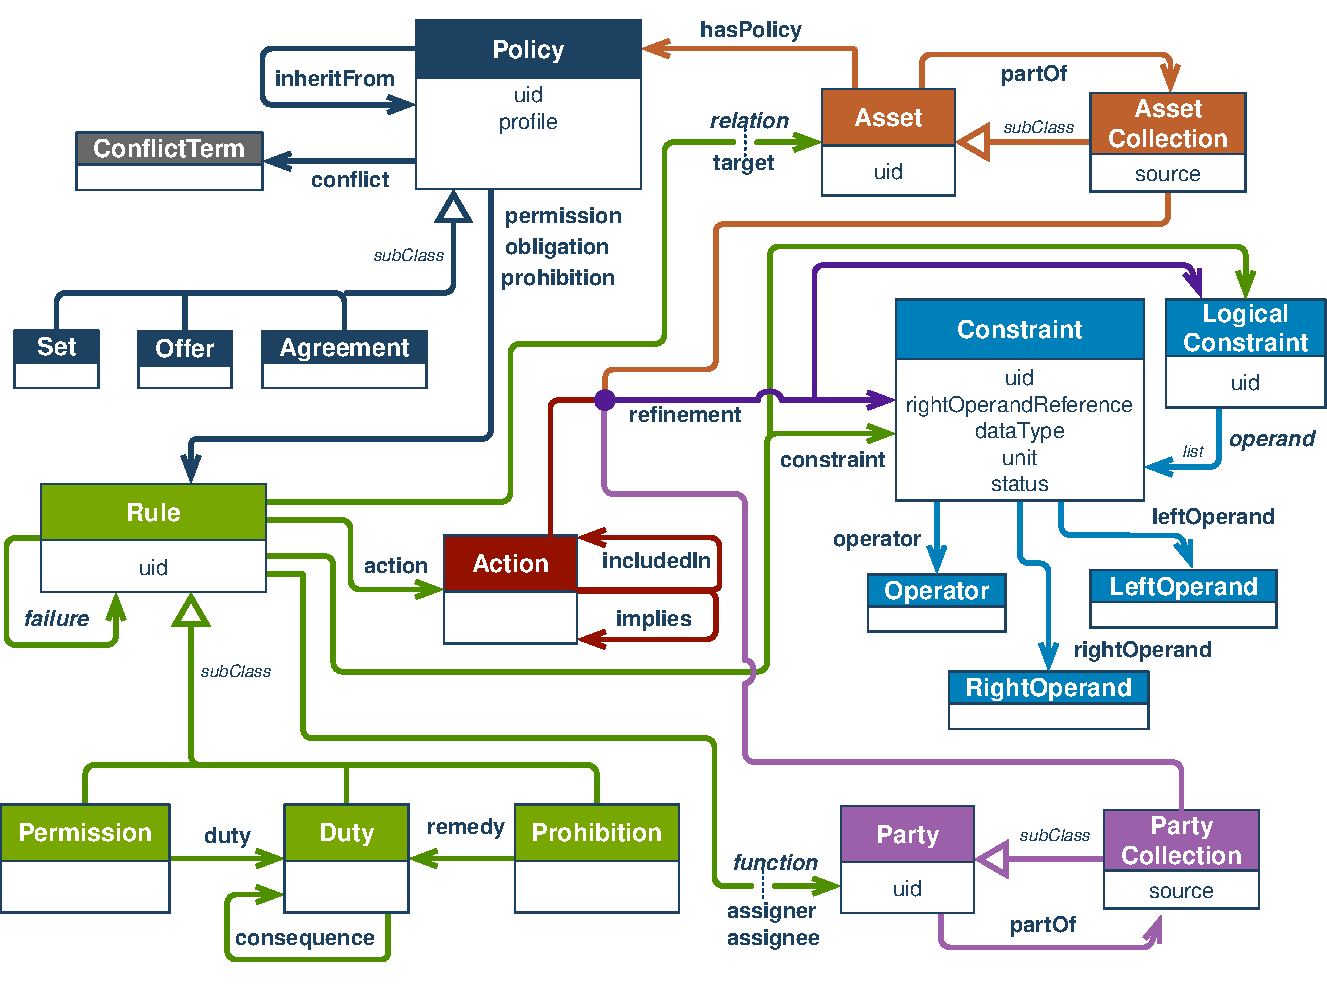
\includegraphics{ODRLModel.pdf}}
	\label{ODRLModelSchema}
	\caption{Schema del modello ODRL\cite{ODRLinfMod}}
\end{figure}
Come visibile all'interno dello schema in figura \ref{ODRLModelSchema}, il modello è basato sulle seguenti entità principali:
\begin{itemize}
	\item \textbf{Policy}: un gruppo di una o più regole;
	\item \textbf{Regola}: concetto astratto che racchiude le caratteristiche comuni di \textbf{permesso}, \textbf{divieto}, \textbf{doveri};
	\item \textbf{Asset}: risorsa o collezione di risorse soggette a regole;
	\item \textbf{Azione}: operazione su un asset;
	\item \textbf{Party}: entità o insieme di entità con un certo ruolo in una regola;
	\item \textbf{Limiti}: espressione logica o booleana imposta su azioni, party, asset o regole.
\end{itemize}
\paragraph{Vocabolari}\mbox{}\\
\label{profili}
``L' \textit{ODRL Vocabulary and Expression} descrive i termini usati dalle policy ODRL e come codificarle''\cite{ODRVocab}. All'interno di ODRL, i vocabolari utilizzati per definire i termini all'interno delle policy vengono detti \textbf{profili}, i quali possono essere usati per definire termini che supportano specifiche applicazioni; all'interno di un profilo è possibile, ad esempio, fornire le specifiche riguardanti nuove sottoclassi di termini già presenti nei vocabolari standard di ODRL. I 2 vocabolari principali definiti sono:
\begin{itemize}
	\item \textbf{ODRL Core Vocabulary}: rappresenta la minima espressione di policy supportata;
	\item \textbf{ODRL Common Vocabulary}: arricchisce il vocabolario precedente con un gruppo di azioni generiche, nuove sottoclassi per le policy, ruoli per i party e relazioni tra gli asset.
\end{itemize}
Una delle principali differenze tra i due vocabolari, la si ha all'interno delle \textbf{azioni} che possono essere indicate: nel primo caso si hanno a disposizione solamente 2 azioni \textbf{use} e \textbf{transfer}, nel secondo caso queste 2 azioni vengono estese da diverse azioni figlie, come mostrato in figura \ref{imgUseTransfer}

\begin{figure}[H]
	\centering
	\def\svgwidth{\columnwidth}
	\scalebox{0.5}{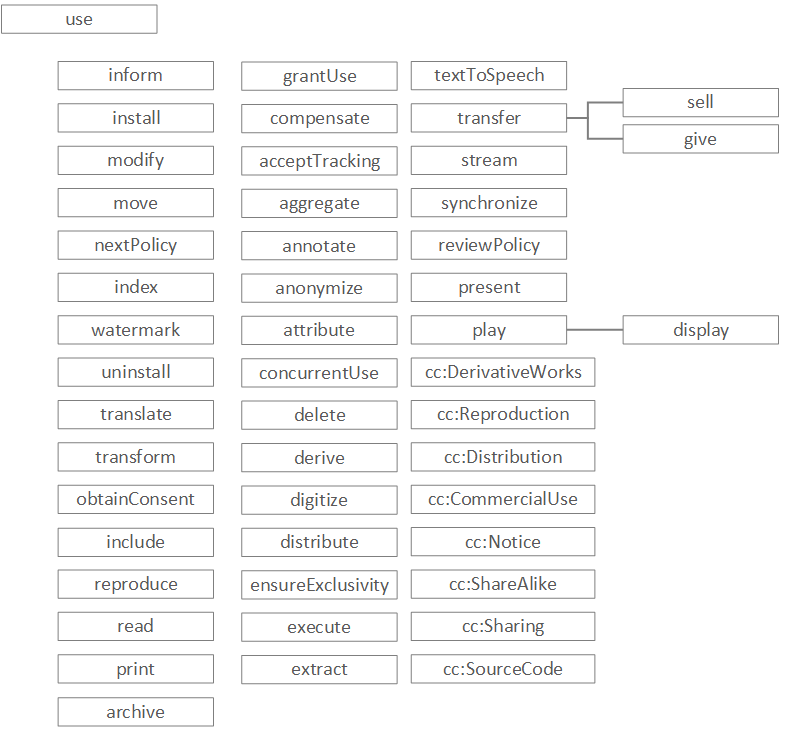
\includegraphics{useTree.png}}
	\label{imgUseTransfer}
	\caption{Tutte le azioni mostrate sono figlie di use, ad eccezioni di trasfer e le sue sottoazioni\cite{ODRLBestPract}}
\end{figure}

\paragraph{Policy}\mbox{}\\
Come definito nel modello presente nella sezione \ref{modello}, una policy è un gruppo non vuoto di \textbf{regole} e, quindi, di \textbf{permessi}, \textbf{divieti} o \textbf{obblighi}. Una policy deve soddisfare i seguenti requisiti:
\begin{itemize}
	\item deve avere un identificativo univoco, detto \textbf{uid};
	\item deve avere almeno una regola;
	\item può specificare un profilo, obbligatorio se non si usa il Core Vocabulary mostrato nella sezione \ref{profili};
	\item può specificare una policy da cui eredita le proprietà;
	\item può specificare una strategia per la risoluzione dei conflitti.
\end{itemize}
Come visibile dalla figura \ref{ODRLModelSchema}, una policy ha 3 prossibili sottoclassi:
\begin{itemize}
	\item \textbf{Set}: un insieme di regole che hanno effetto;
	\item \textbf{Agreement}: regole concesse ad una entità assegnataria da una assegnatrice;
	\item \textbf{Offer}: proposta di una regola da parte di un assegnatore.
\end{itemize}
Di seguito un esempio di policy definita mediante ODRL:
\begin{lstlisting}[language=json,firstnumber=1,caption={Policy con sottoclasse \textbf{Set}},captionpos=b,label=esmpioPolicy]
{
 "@context": "http://www.w3.org/ns/odrl.jsonld",
 "@type": "Set",
 "uid": "http://example.com/policy:1010",
 "permission": [{
   "target": "http://example.com/asset:9898.movie",
   "action": "use"
 }]
}
\end{lstlisting}
La policy mostrata nel listing \ref{esmpioPolicy} presenta i campi:
\begin{itemize}
	\item @type: serve ad indicarne la sottoclasse;
	\item @context : serve ad indicare che il file deve essere conforme ad ODRL, rappresentato dall'URL da cui si può ottenere l'ODRL Common Vocabulary\cite{ODRLCV};
	\item nel contesto sono presenti altri link per le altre proprietà, ad esempio quello per la descrizione di \textit{Set} e per \textit{use};
	\item non usando termini fuori dai 2 vocabolari principali, non necessita la definizione di un profilo;
	\item l'id univoco è rappresentato da un URL con le informazioni relative alla risorsa;
\end{itemize}
\bibliography{cit}{}
\bibliographystyle{plain}
\end{document}